\documentclass[M3_Night6_Solutions]{subfiles}

\IfSubStr{\jobname}{\detokenize{Solutions}}{\toggletrue{solutions}}{\togglefalse{solutions}}

\fancypagestyle{firstpage}

{\rhead{Night 6 \linebreak \textit{Version: \today}}}

\title{Night 6: Frames of Reference and LIDAR}
\author{Quantitative Engineering Analysis}
\date{Spring 2019}

\begin{document}

\maketitle
\thispagestyle{firstpage}

\section{Overview}
In this overnight activity you are going to think about transforming points between different frames of reference, and how to apply this data collected by the LIDAR on the NEATO in order to create a "map" of the room.

In many ways, this material is not new, but it will feel new. This activity draws heavily on the translation and rotation matrices developed in Module 2, along with the polar coordinate material from earlier in Module 3. However, rather than translating and rotating points, we will be using translation and rotation matrices to express points in different frames of reference.

Unfortunately, we have not found anything particularly useful online to help, so we have tried to write a pretty self-contained set of notes. Here are the key points that we will discuss:

\begin{myboxi}[Key Points]
\bi
\item A frame of reference is defined by an origin and a coordinate system.
\item A coordinate system is defined by a set of basis vectors.
\item The coordinates of a point correspond to the components along each basis vector of a position vector from the origin to the point.
\item The coordinates of a point are therefore dictated by the frame of reference.
\item The notation $\r_G$ or $(x,y)_G$ refers to the coordinates of a point in frame G.
\item Points can be transformed from one frame to another using matrix multiplication.
\item If frame M has origin located at $(a,b)_G$, and has basis vectors rotated counterclockwise by $\theta$, then the transformation from frame G to frame M is
\[ \r_M = \R_{MG} \T_{MG} \r_G \]
where $\T_{MG}$ is the matrix that translates the origin of frame G to frame M, and $\R_{MG}$ is the matrix that rotates the basis vectors of frame G to frame M:
\[\R_{MG} = \threebythree{\cos \theta}{\sin \theta}{0}{-\sin \theta}{\cos \theta}{0}{0}{0}{1} \]
\[\T_{MG} = \threebythree{1}{0}{-a}{0}{1}{-b}{0}{0}{1} \]
\item Transforming back from frame M to frame G involves the inverse of these matrices
\[ \r_G = \T_{MG}^{-1} \R_{MG}^{-1} \r_M \]
\item These concepts and quantities can be used to transform LIDAR data to the room frame in order to create a map.
\ei
\end{myboxi}

\clearpage

\section{Frames of Reference [2 Hrs]}

In robotics and indeed many other applications, it is often useful to express points using different coordinate systems. You have already done this to a certain extent in Module 2 when you expressed vectorized images as linear combinations of eigenfaces. In robotics applications, it is beneficial to express points relative to a fixed origin (e.g. a point designated as the origin in a room) and orthogonal basis vectors. In other cases, it is convenient to express points relative to an origin on the robot itself, with one basis vector in the direction of motion, and the others in orthogonal directions. Here, we will first develop some tools to translate points from one coordinate system to another, and apply these tools in the context of the NEATO. You will then be able to take points expressed in a coordinate system centered on the robot (e.g. from sensor data), and represent them in terms of an fixed coordinate system (e.g. with a corner of a room as the origin). We will work in 2D, but we can just as easily extend this discussion to higher dimensions.

\subsection{Coordinate Systems with the same Origin}

A coordinate system consists of an {\bf origin} and a set of {\bf basis vectors}. Recall that a set of vectors form a basis if they are linearly independent---if they are mutually orthogonal then we have an orthogonal coordinate system.

The standard basis vectors for 2D are usually labelled $\ihat$ and $\jhat$, but they are sometimes written as $\e_1$ and $\e_2$, or $\e_x$ and $\e_y$, or $\hat{\x}$ and $\hat{\y}$. From now on, we will assume that the global reference frame (frame G) is defined by the standard basis vectors, but just to be very clear we will use a subscript and write $\ihat_G$ and $\jhat_G$ as the basis vectors of the global frame G.


Points in 2D are expressed in terms of the basis vectors, and we refer to the component of the vector as the {\bf coordinates} of the point. For example, the point A in Figure 1 has coordinates $(4,3)$ when expressed in terms of the standard basis vectors. We might also write the position vector of $A$ as

\begin{marginfigure}
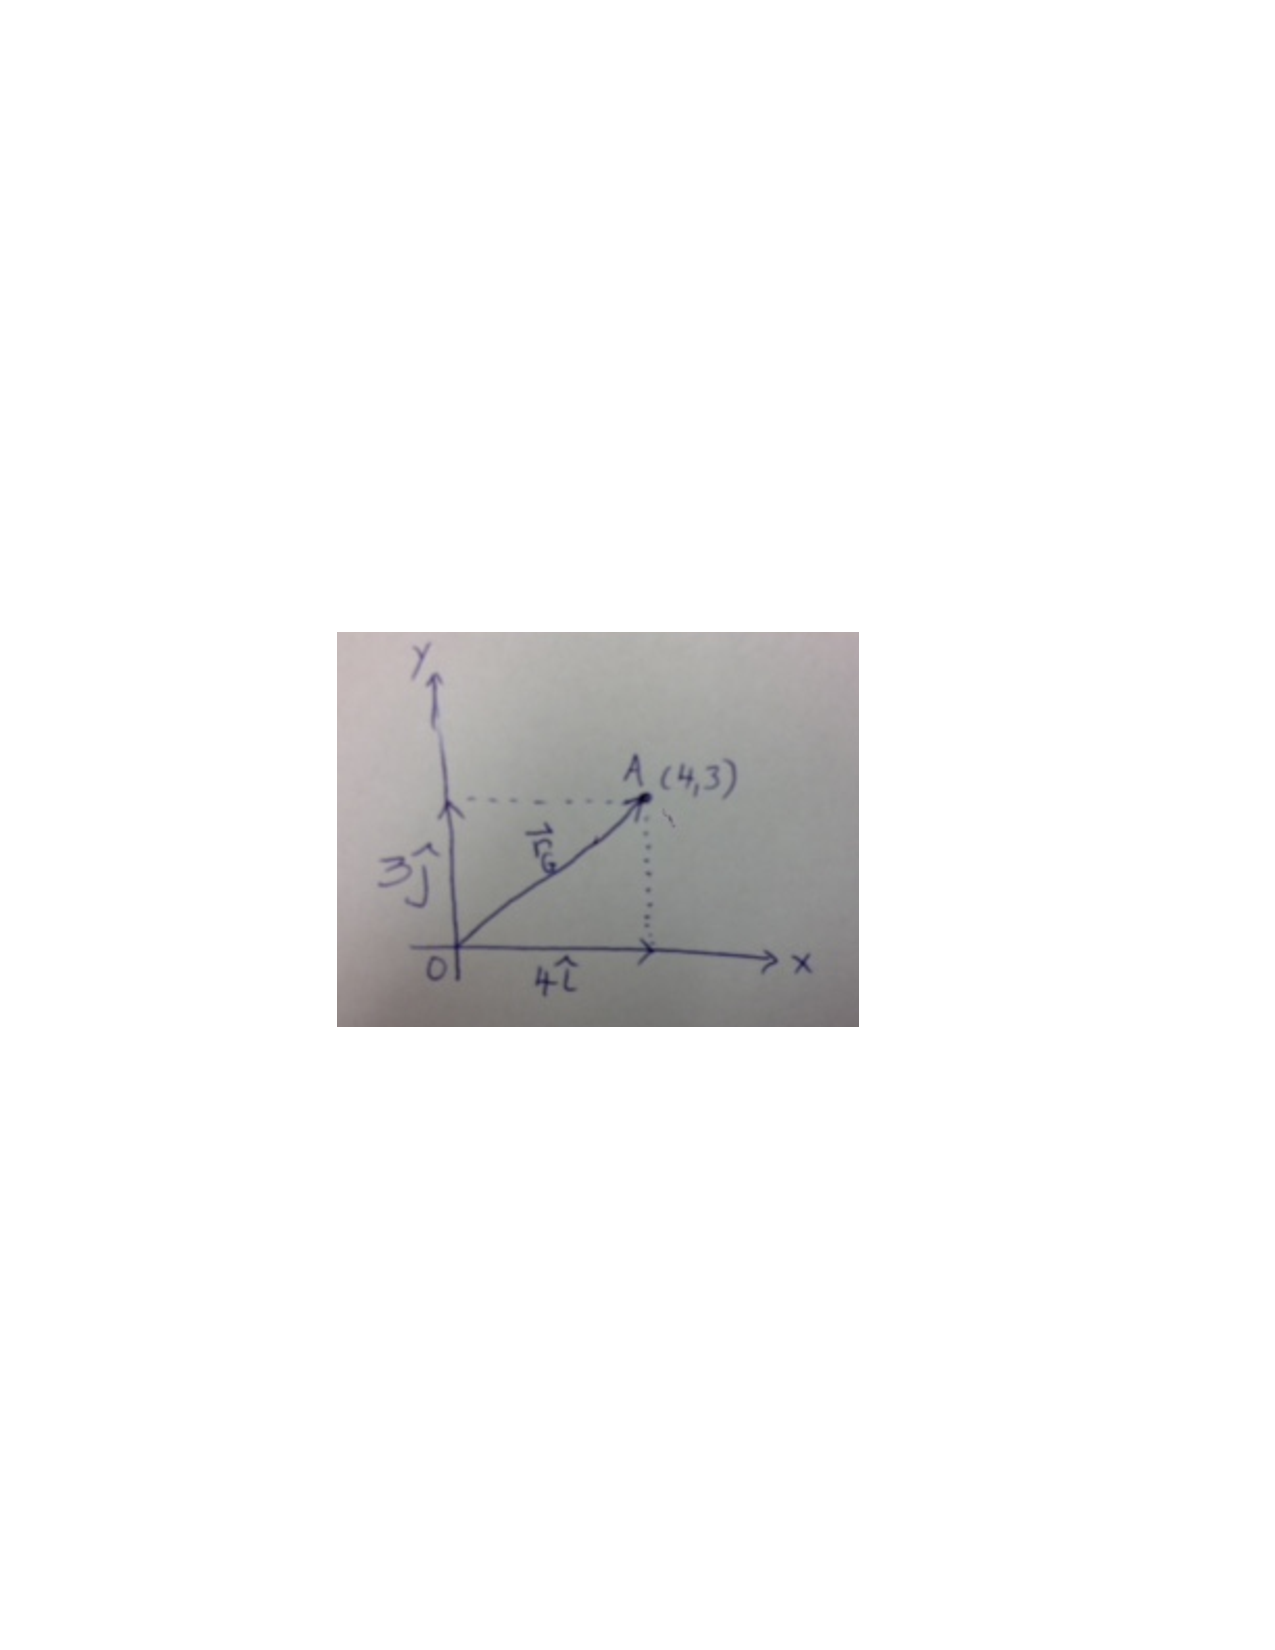
\includegraphics[width=2.5in]{figs/globalframe.pdf}
\caption{The coordinates of the point $(4,3)$ are the projections of the position vector onto the relevant basis vectors.}
\label{fig:globalframe}
\end{marginfigure}

\[\r_G = 4 \ihat_G + 3 \jhat_G \]
or express it as a row or column vector
\[\r_G = \twobyone{4}{3} \]
All of these refer to the same point, but the first and last representations imply the basis vectors, while the second representation makes it explicit. We use the notation $\r_G$ to be clear that this is the position vector of point $A$ when expressed in the frame G. Notice that the coordinates $(x_G,y_G)$ of the point A are simply the projection of the position vector onto the relevant basis vectors,
\[x_G = \r_G \cdot \ihat_G, \; y_G = \r_G \cdot \jhat_G \]
Since these basis vectors are mutually orthogonal the coordinates are simply $(4,3)$ as expected, but again for clarity we will write $(4,3)_G$ to mean that these are the coordinates in the frame G.

How do we express the same point in terms of a new set of basis vectors, $\ihat_M$ and $\jhat_M$?  Mathematically, we are trying to express the vector $\r_M$ as a linear combination of these vectors
\[ \r_M = \x_M \ihat_M + y_M \jhat_M \]
where the coordinates of the point are now $(x_M,y_M)$, i.e. the x and y coordinates of the point in the frame of reference M. See Figure 2.

\begin{marginfigure}
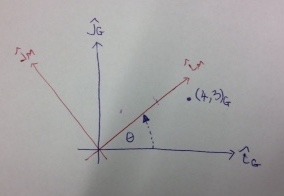
\includegraphics[width=2.5in]{figs/newframe}
\caption{The frame M has the same origin, but the basis vectors are rotated by an angle of $\theta$. The coordinates of the point $(4,3)_G$ can be expressed in terms of the new frame M.}
\label{fig:globalframe}
\end{marginfigure}

The components of the point A expressed in this coordinate system is again the projection of the position vector in the frame G onto each basic vector of frame M in turn,
\[x_M = \r_G \cdot \ihat_M, \; y_M = \r_G \cdot \jhat_M \]
Since $\r_G = x_G \ihat_G + y_G \jhat_G$ we see that
\[x_M = x_G \ihat_G \cdot \ihat_M + y_G \jhat_G \cdot \ihat_M, \; y_M = x_G \ihat_G \cdot \jhat_M + y_G \jhat_G \cdot \jhat_M\]
Whilst this looks cumbersome, it becomes a lot clearer when we use the following matrix-vector formulation
\[\twobyone{x_M}{y_M} = \twobytwo{\ihat_G \cdot \ihat_M}{\jhat_G \cdot \ihat_M}{\ihat_G \cdot \jhat_M}{\jhat_G \cdot \jhat_M} \twobyone{x_G}{y_G}\]
This matrix is the transformation matrix from the global reference frame (frame G) to the new reference frame (frame M), and we will often use the notation $\R_{MG}$ when referring to this transformation matrix
\[\r_M = \R_{MG} \r_G \]

For example, consider the frame M shown in Figure 2, which is simply the global frame rotated counter-clockwise by an angle $\theta$. The basis vectors in this frame are
\[ \ihat_M = \twobyone{\cos \theta}{\sin \theta}, \; \jhat_M = \twobyone{-\sin \theta}{\cos \theta} \]
which means that the transformation matrix from frame G to frame M is
\[\R_{MG} = \twobytwo{\cos \theta}{\sin \theta}{-\sin \theta}{\cos \theta} \]
which is almost identical to the rotation matrix we met in Module 2. Rather than rotating the point through $\theta$ degrees, it rotates the coordinate system through $\theta$ degrees and expresses the point in terms of this new coordinate system. If $\theta = \pi/4$, the point $(4,3)_G$ is expressed as
\begin{eqnarray*}
\r_M &=& \twobytwo{1/\sqrt{2}}{1\sqrt{2}}{-1/\sqrt{2}}{1/\sqrt{2}} \twobyone{4}{3} \\
\Rightarrow \r_M &=& \twobyone{7/\sqrt{2}}{-1/\sqrt{2}}
\end{eqnarray*}
or equivalently $(7/\sqrt{2},-1/\sqrt{2})_M$.

What if we have the coordinates of a point in frame M, and we wish to express them in frame G? Referring to the transformation matrix we developed earlier, we can express this using the matrix inverse
\[\r_G = \R_{MG}^{-1} \r_M \]
Since this inverse must be the transformation that takes points from frame M to frame G it must be true that
\[\R_{GM} = \R_{MG}^{-1} \]
Transforming from frame M to frame G corresponds to a clockwise rotation of $\theta$ so that $\R_{GM}$ must be the transpose of $\R_{MG}$,
\[\R_{GM} = \twobytwo{\cos \theta}{-\sin \theta}{\sin \theta}{\cos \theta} \]
For example, consider the point $(1,2)_M$ in frame M. The coordinates of this point in frame G must be
\begin{eqnarray*}
\r_G &=& \twobytwo{1/\sqrt{2}}{-1\sqrt{2}}{1/\sqrt{2}}{1/\sqrt{2}} \twobyone{1}{2} \\
\Rightarrow \r_G &=& \twobyone{-1/\sqrt{2}}{3/\sqrt{2}}
\end{eqnarray*}
or simply $(-1/\sqrt{2},3/\sqrt{2})_G$.

% in the first problem block, make sure to use the series option for enumerate
\begin{enumerate}[series=exercises, label=\textbf{Exercise} (\arabic*)]
\item The frame M is a counterclockwise rotation of the global frame G by $\pi/3$ radians.
\be
\item Draw the basis vectors for frame G and frame M.
\item Plot the frame G coordinates $(2,-1)_G$. Now express the frame G coordinates $(2,-1)_G$ in the frame M, and confirm that this is the same point by plotting it using the frame M.
\item Plot the frame M coordinates $(3,-2)_M$. Now express the frame M coordinates $(3,-2)_M$ in the frame G, and confirm that this is the same point by plotting it using the frame G.
\ee
\solution{
\begin{figure}
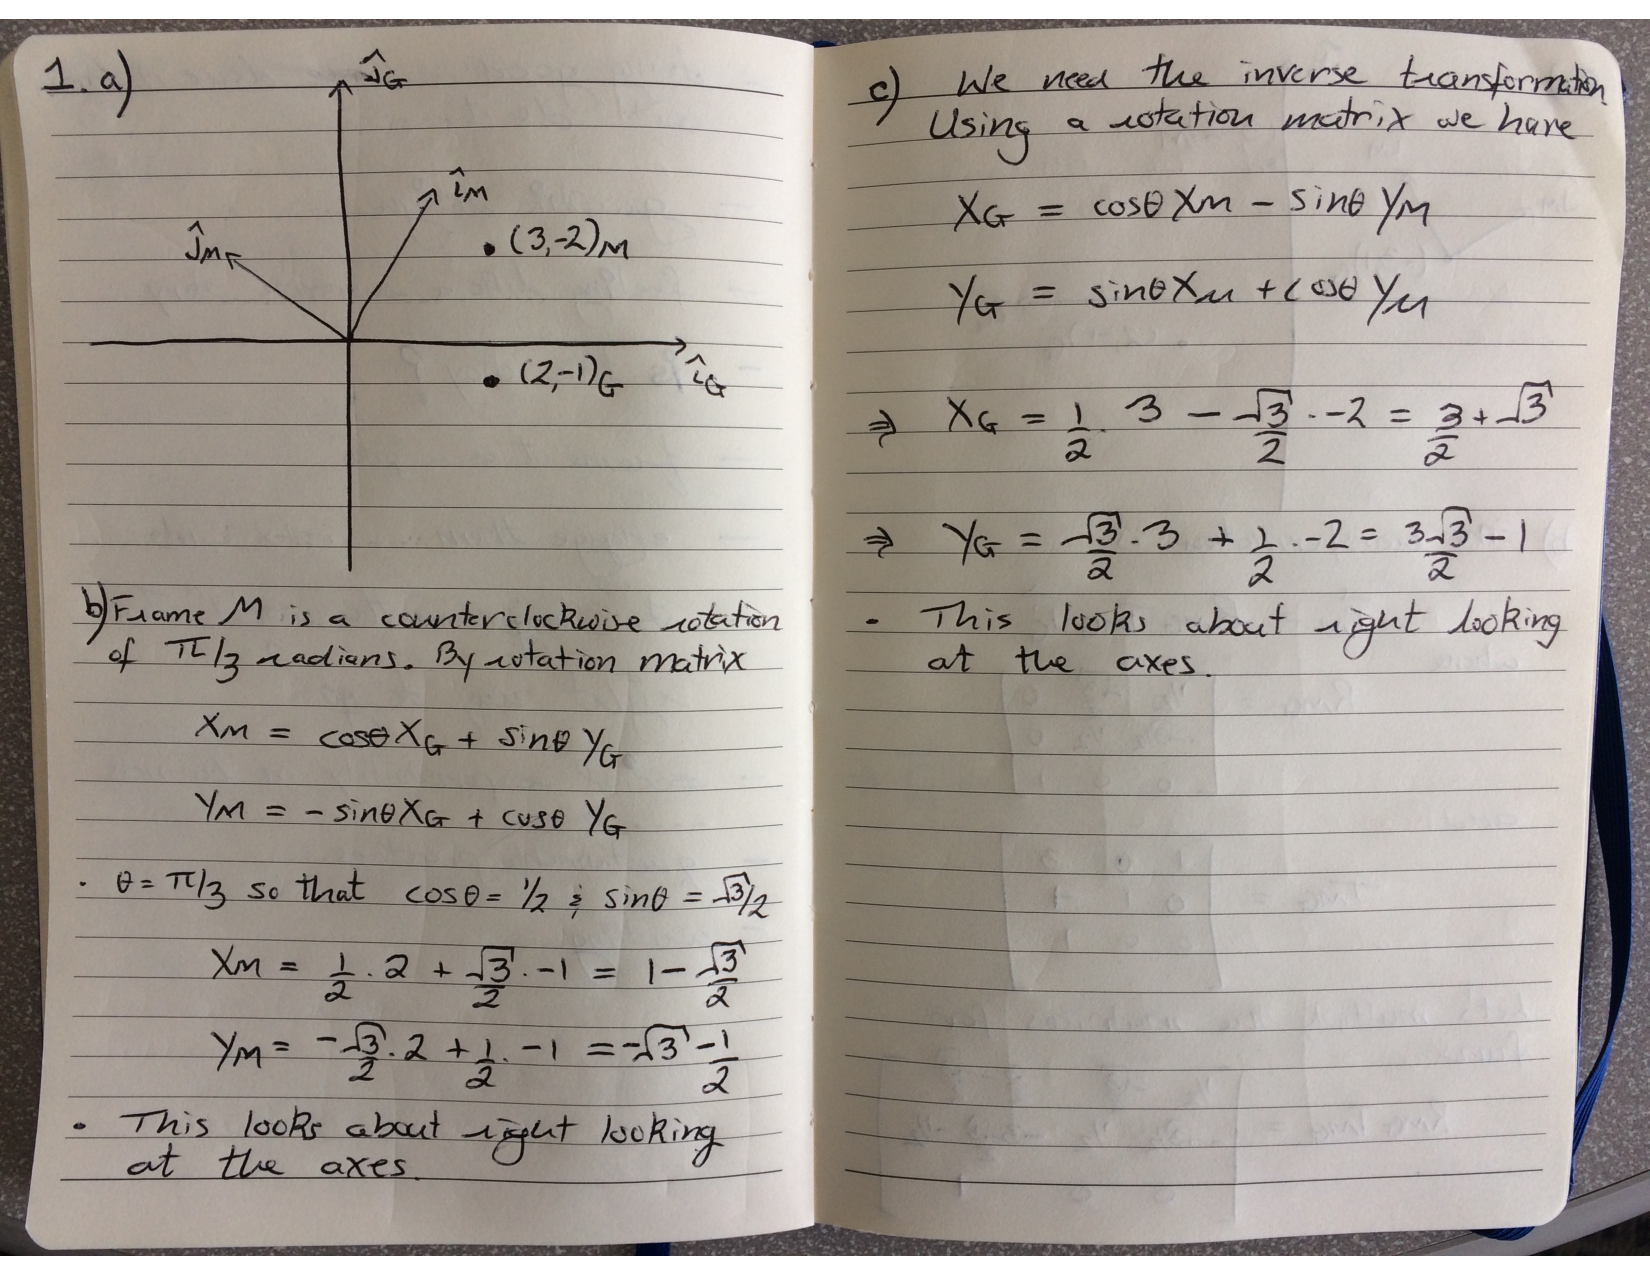
\includegraphics[width=12cm]{figs/sol1abc}
\end{figure}
}
\ee


\subsection{Coordinate Systems with a different Origin}

In addition to defining new basis vectors, we often encounter situations in which we use a new origin. In Figure 3 we define a global frame with basis vectors $\ihat_G$ and $\jhat_G$, and origin $O_G$. We also define a frame M with basis vectors $\ihat_M$ and $\jhat_M$, and origin $O_M$. How do we transform points from frame G to frame M, and vice versa?

Fortunately, we already met the concept of translating points in Module 2, and here we will utilize these ideas to translate the origin before rotating the basis vectors.  Recall from Module 2 that in order to translate a point we can use the translation matrix
\[\T = \threebythree{1}{0}{t_x}{0}{1}{t_y}{0}{0}{1} \]
where $t_x$ and $t_y$ are the components of the translation, and the translation matrix acts on the vector
\[\threebyone{x}{y}{1} \]

For example, let's consider the case when the origin of frame M is located at $(a,b)_G$. The coordinates of this point in frame M must be, by definition, $(0,0)_M$. The components of the translation must therefore be $-a$ and $-b$ and the translation matrix that moves the origin of frame G to frame M is then
\[\T_{MG} = \threebythree{1}{0}{-a}{0}{1}{-b}{0}{0}{1} \]
and the translation matrix that moves the origin of frame M to frame G
\[\T_{GM} = \threebythree{1}{0}{a}{0}{1}{b}{0}{0}{1} \]
In order to be consistent, we should adapt our rotation matrix so that it acts on a vector with $1$ in the third slot
\[\R_{MG} = \threebythree{\cos \theta}{\sin \theta}{0}{-\sin \theta}{\cos \theta}{0}{0}{0}{1} \]
and
\[\R_{GM} = \threebythree{\cos \theta}{-\sin \theta}{0}{\sin \theta}{\cos \theta}{0}{0}{0}{1} \]

\begin{marginfigure}
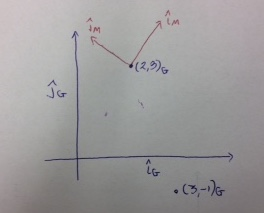
\includegraphics[width=2.5in]{figs/newnewframe}
\caption{The frame M has an origin at $(2,3)_G$, and the basis vectors are rotated by an angle of $\theta$. The coordinates of the point $(3,-1)_G$ can be expressed in terms of the new frame M.}
\label{fig:globalframe}
\end{marginfigure}

We are now ready to transform a point from frame G to frame M, by first translating the origin of frame G to the origin of frame M, and then rotating the basis vectors from frame G to frame M. The position vector of an arbitrary point is then
\[\r_M = \R_{MG} \T_{MG} \r_G \]
We can, if we choose, combine the translation with the rotation into a general transformation, but we don't have to, and there are some advantages to keeping the distinction clear. 

Transforming back from frame M to frame G would be accomplished with
\begin{eqnarray*}
\r_G &=& (\R_{MG} \T_{MG})^{-1} \r_M \\
\Rightarrow \r_G &=& \T_{MG}^{-1} \R_{MG}^{-1} \r_M
\end{eqnarray*}
We've already seen that the inverse of the rotation matrix is just the transpose of the original and thus $(\R_MG)^{-1} = R_{GM}$. This makes sense. To rotate back from frame M to frame G we use the $R_{GM}$. Furthermore, the inverse of the translation matrix $\T_{MG}$ is just the translation matrix $\T_{GM}$. Notice, however, that we first apply the inverse rotation and then the inverse translation,
\[\r_G = \T_{GM} \R_{GM} \r_M \]

For example, let's express the point $(3,-1)_G$ in frame M, which has its origin at $(2,3)_G$, with basis vectors rotated counterclockwise by $\pi/4$. The coordinates in frame M are therefore
\begin{eqnarray*}
\r_M &=& \threebythree{1/\sqrt{2}}{1/\sqrt{2}}{0}{-1/\sqrt{2}}{1/\sqrt{2}}{0}{0}{0}{1} \threebythree{1}{0}{-2}{0}{1}{-3}{0}{0}{1} \threebyone{3}{-1}{1} \\
\Rightarrow \r_M&=& \threebythree{1/\sqrt{2}}{1/\sqrt{2}}{0}{-1/\sqrt{2}}{1/\sqrt{2}}{0}{0}{0}{1} \threebyone{1}{-4}{1} \\\Rightarrow \r_M
&=& \threebyone{-3/\sqrt{2}}{-5/\sqrt{2}}{1}
\end{eqnarray*}
which means the coordinates are $(-3/\sqrt{2},-5/\sqrt{2})_M$. Let's check to see if we can transform this point back from frame M to frame G. The coordinates in frame G are therefore
\begin{eqnarray*}
\r_G &=& \threebythree{1}{0}{2}{0}{1}{3}{0}{0}{1}   \threebythree{1/\sqrt{2}}{-1/\sqrt{2}}{0}{1/\sqrt{2}}{1/\sqrt{2}}{0}{0}{0}{1} \threebyone{-3/\sqrt{2}}{-5/\sqrt{2}}{1} \\
\Rightarrow \r_G&=& \threebythree{1}{0}{2}{0}{1}{3}{0}{0}{1} \threebyone{1}{-4}{1} \\
\Rightarrow \r_G &=& \threebyone{3}{-1}{1}
\end{eqnarray*}
which is just where we started!

% when adding a second block of problems make sure to use "resume" instead of "series"
\begin{enumerate}[resume=exercises, label=\textbf{Exercise} (\arabic*)]
\item The frame M is a counterclockwise rotation of the global frame G by $\pi/3$ radians, and has its origin at $(-3,1)_G$.
\be
\item Draw the origin and basis vectors for frame G and frame M.
\item Plot the frame G coordinates $(2,-1)_G$. Now express the frame G coordinates $(2,-1)_G$ in the frame M, and confirm that this is the same point by plotting it using the frame M.
\solution{
\begin{figure}
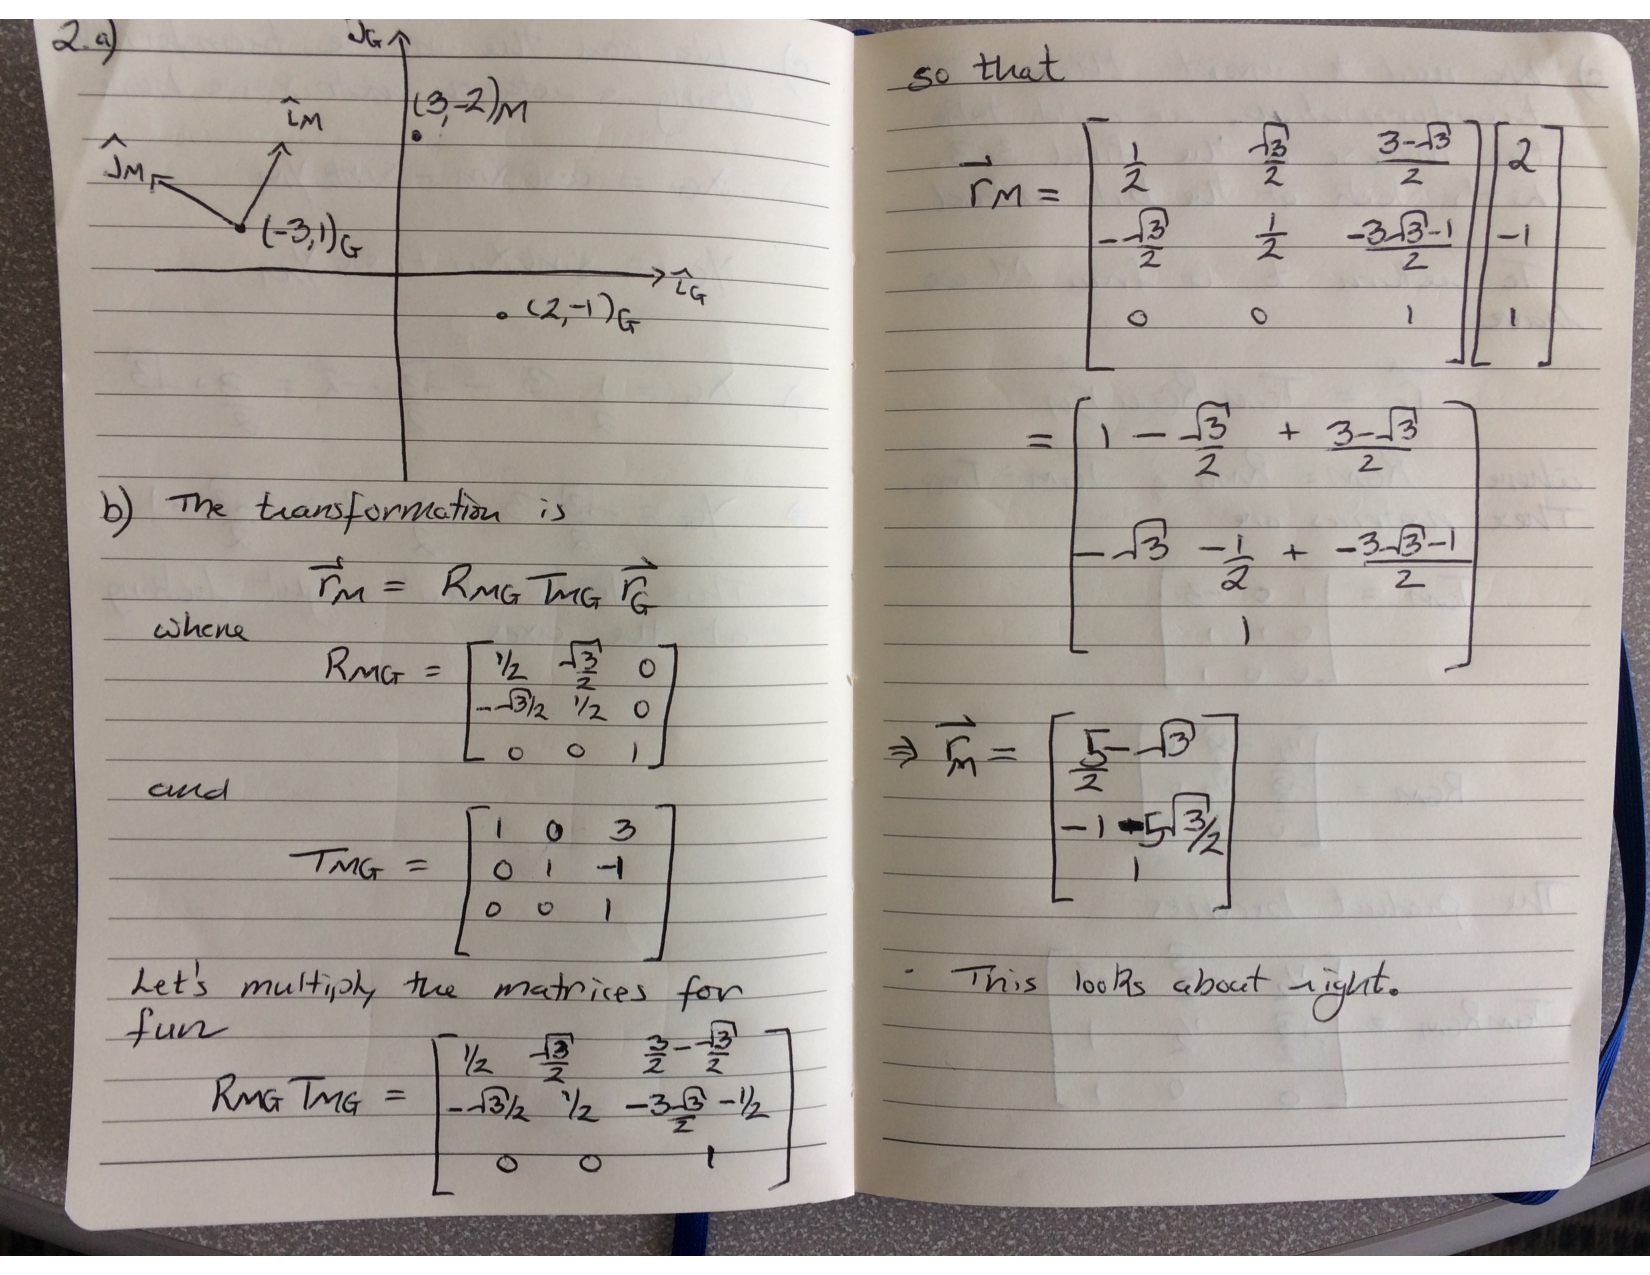
\includegraphics[width=12cm]{figs/sol2ab}
\end{figure}
}
\item Plot the frame M coordinates $(3,-2)_M$. Now express the frame M coordinates $(3,-2)_M$ in the frame G, and confirm that this is the same point by plotting it using the frame G.
\solution{
\begin{figure}
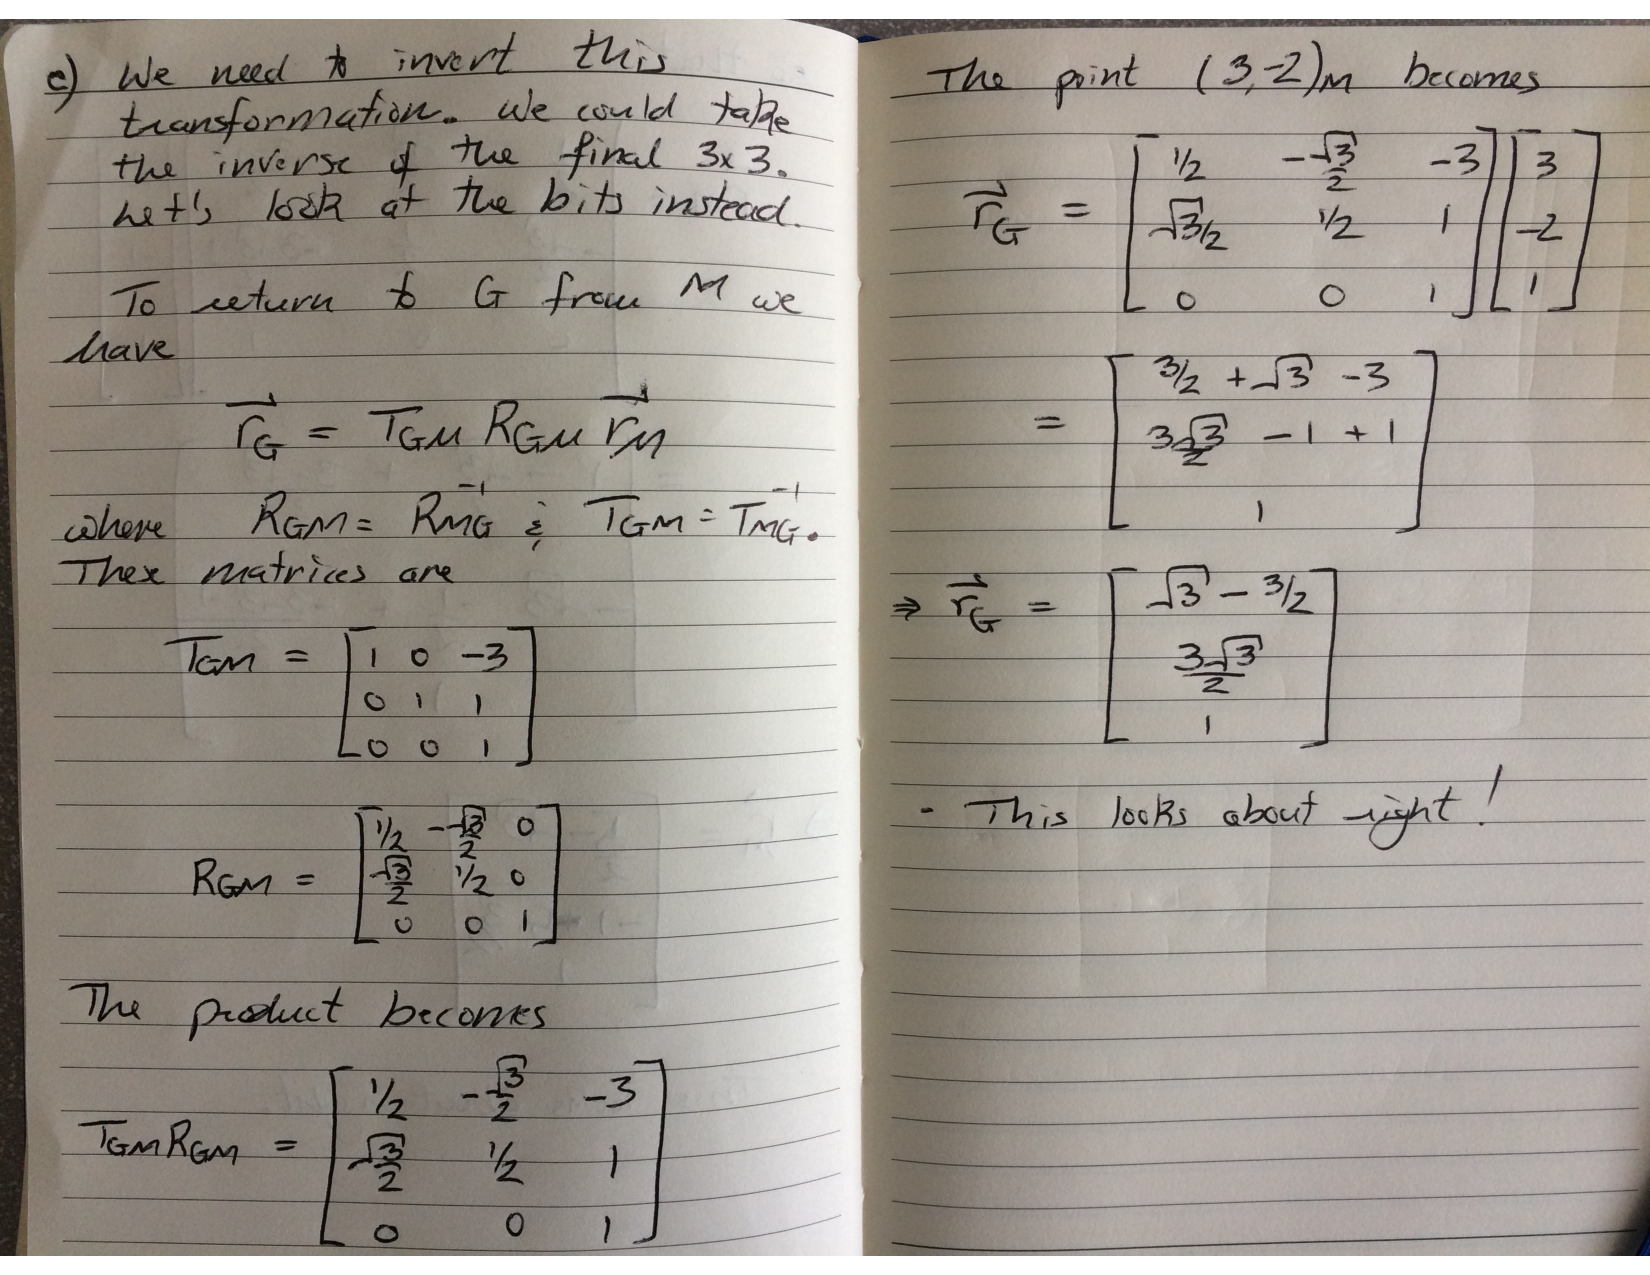
\includegraphics[width=12cm]{figs/sol2c}
\end{figure}
}
\ee
\ee

\clearpage

\section{Application to the NEATO [2 Hrs]}

\begin{marginfigure}
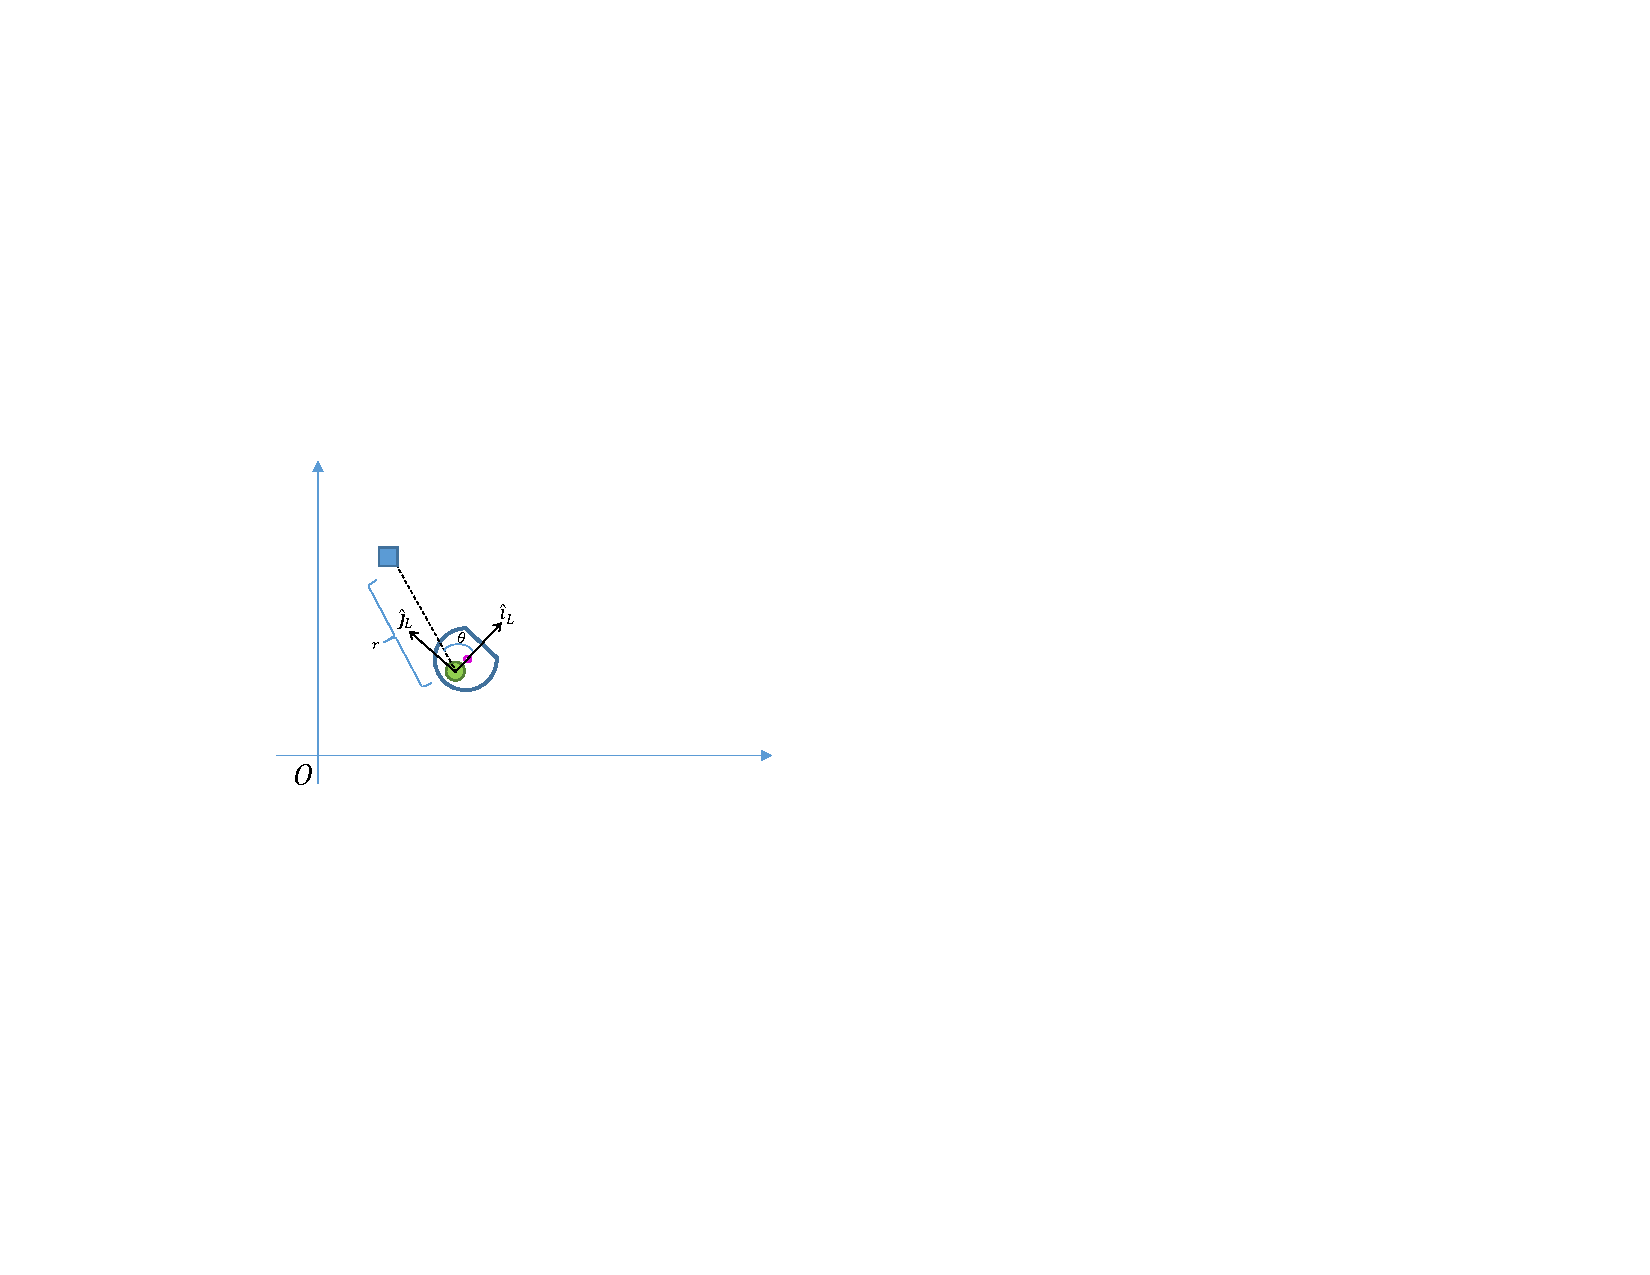
\includegraphics[width=2.5in]{figs/NeatoCoordinateFrame.pdf}
\caption{Illustration of NEATO with different coordinate systems with origin at the center of rotation of the LIDAR, and in the origin of a fixed frame of reference (e.g. origin of the room).}
\label{fig:NeatoAngles}
\end{marginfigure}
The LIDAR reading provides a range and angle with respect to the center of rotation of the LIDAR sensor on the NEATO, with the angle measured relative to the front of the NEATO as illustrated by $\theta$ in Figure \ref{fig:NeatoAngles}. The square object is located at a distance $r$ and angle $\theta$  as measured by the LIDAR on the Neato. 

\begin{marginfigure}
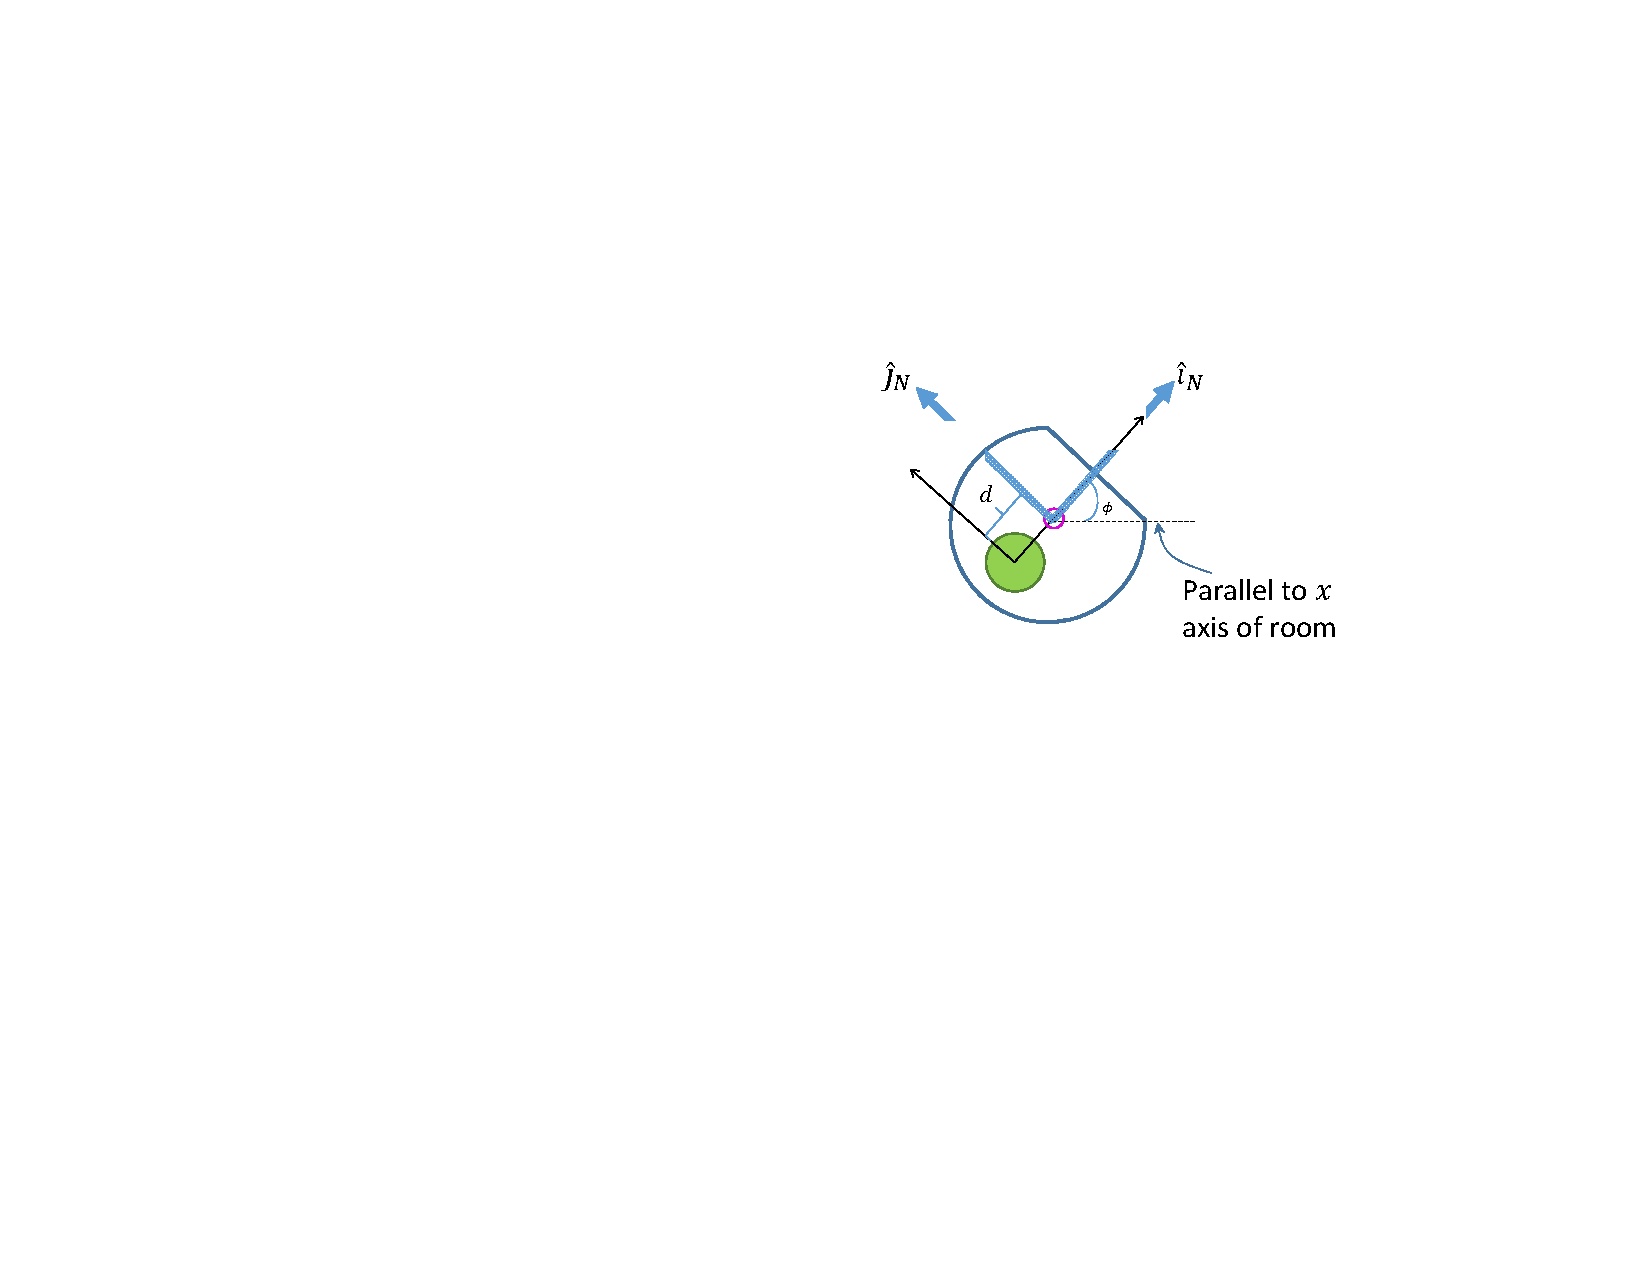
\includegraphics[width=2.0in]{figs/NeatoFrameZoom.pdf}
\caption{Illustration of NEATO with origin at center of rotation.}
\label{fig:Neato}
\end{marginfigure}

For further reference, consider Figure \ref{fig:Neato} which indicates the location of the LIDAR relative to the center of rotation of the Neato. The center of rotation of the Neato is indicated by the magenta circle and is the origin of two orthogonal unit vectors $\ihat_N$ and $\jhat_N$ (thicker, light blue arrows). You can physically measure the distance \textit{d} between the origin of the reference frame based on the LIDAR and the origin of the reference frame based on the Neato's center of rotation.

The orientation of the Neato relative to the absolute horizontal axis of the room is indicated by the angle $\phi$. Depending on your application, you may wish to express the position of the object (the box, in this case) in terms of a coordinate system relative to the center of rotation of the LIDAR sensor with unit vectors $\ihat_L$ and $\jhat_L$, center of rotation of the Neato with the unit vectors $\ihat_N$ and $\jhat_N$, or the global frame of reference indicated by the origin marked "O" and the blue arrows for which the unit vectors are $\ihat_G$ and $\jhat_G$.

\begin{enumerate}[resume=exercises, label=\textbf{Exercise} (\arabic*)]
\item Suppose that the LIDAR returns a value of $(r, \theta)$ when scanning an object. With reference to Figure \ref{fig:NeatoAngles}, please express the location of the object with respect to the LIDAR frame L.
\solution{We will denote the location of the object in the LIDAR frame L as $\r_L$.  If we measure the polar coordinates of the object then its location is $\r_L = \twobyone{r \cos \theta}{r \sin \theta}$.}
\item With reference to Figures \ref{fig:NeatoAngles} and \ref{fig:Neato}, please express the location of the object with respect to the NEATO frame N.
\solution{We will denote the location of the object in the NEATO frame as $\r_N$. It is a translation with respect to the LIDAR origin. The location of the object is now $\r_N = \twobyone{r \cos \theta -d}{r \sin \theta}$.}
\item Please express the location of the square object in the global frame G. Assume that the center of rotation of the NEATO is located at $(x_N, y_N)_G$.
\solution{The NEATO is translated and rotated with respect to the room. The transformation matrices are
\[ \T_{GN} = \threebythree{1}{0}{x_N}{0}{1}{y_N}{0}{0}{1} \]
\[\R_{GN} = \threebythree{\cos \phi}{-\sin \phi}{0}{\sin \phi}{\cos \phi}{0}{0}{0}{1} \]
Multiplying these out and transforming the coordinates of the object in the NEATO frame leads to
\[ \r_G = \twobyone{r \cos (\theta+\phi) - d \cos \phi + x_N}{r \sin (\theta+\phi) - d \sin \phi + y_N} \] 
where we have used a trig formula.
}
    
\item Now, we will use these techniques to take LIDAR data and build a map with respect to a fixed co-ordinate frame. In the classroom, we have defined an origin, $x$, and $y$ axes, as well as placed objects on the floor at fixed locations in the  Gauntlet. \textbf{Your job is to build a map of the  Gauntlet when the NEATO is placed at different positions and orientations.} The map will be built using the co-ordinate frame with the origin as marked in the Gauntlet and unit vectors in the $x$ and $y$ directions.     We shall call this the Fixed (or Global) coordinate frame.
 Recall that the LIDAR data is provided to you in polar co-ordinates using the co-ordinate frame with the origin at the center of the LIDAR sensor and the basis vectors pointing in the forward direction of the LIDAR, and $90^0$ counter-clockwise from it.
    
    \be
    \item Read through the parts (b)-(e) below. For the sake of logistics, you can collect all of your data (four different placements of the Neato) and then construct the plots.  You can use the code in \href{https://drive.google.com/file/d/1ZnDro0H-HyNaas_lySvk0eZ_NxsUCME9/view?usp=sharing}{collectAScan.m} or write your own code to collect these data. Remember to record your measurement of the position and orientation of the Neato after each time you move it. 
    \item Place the NEATO at the origin facing in the direction of the $x$ axis and collect data from the LIDAR. Express the LIDAR data in the fixed co-ordinate frame. Plot the data in MATLAB using the fixed reference frame and compare it to the locations of the objects in the Gauntlet.
        
    \item With the NEATO at the origin, rotate it through some angle $\phi$ (you can just pick your favourite angle here) and repeat what you did for the previous part (i.e., collect LIDAR data, translate to the fixed co-ordinate frame, plot in MATLAB, compare to the locations of the physical objects in the Gauntlet).  Just to make sure we are crystal clear, when we say to rotate the Neato you can either do this by literally picking the Neato up and rotating it, or you can do it by sending the Neato relevant motor command (e.g., using \emph{teleopAndVisualizer.m}).
        
    \item Now, move the NEATO to a different location (pick your favourite location in the Gauntlet), but keep it pointing in the same direction as the $x$ axis, and repeat what you did for the previous part.  You could either use wheel encoder data or take physical measurements here to determine the position and orientation of the NEATO.
        
    \item Now, move the NEATO to a different location and pointing in some arbitrary direction, and repeat what you did for the previous part.  
    \ee
    
\ee


\end{document}
